% \newpage para arrancar una pagina nueva
% \mbox y \ fbox para evitar que te corte al medio una palabra que vos querer tenr toda junta
% \mbox{} se puede usar cuando 2 letras se pegan. entonces lo ponemos entre medio de esas 2 letras
% The \part command does not influence the numbering sequence of chapters.
% \footnote{footnote text} para poner notas al pie de la pagina
% \underline{text}
% \emph{text} pone en italica
% \begin{enumerate} o {itemize} y despues listas con \item o {description} y listas con \item[palabra]



\documentclass[a4paper,10pt, notitlepage]{article}
\usepackage[utf8x]{inputenc}
\usepackage[english,spanish]{babel}

\usepackage{graphicx}
\usepackage{verbatim}

\pagestyle{plain} %o pagestyle{plain} , valor defecto   {headings}
% define the title
\title{\textbf{TP0 Organización de las Computadoras (66.20)}}
% \author{Rodriguez Genaro, Leandro \and Padron: 92098 \\ 
\author{}
\date{}


\begin{document}
% generates the title
\maketitle

\begin{center}
Grupo Nro. X - 1er. Cuatrimestre de 2012                  \\
66.20 Organización de Computadoras                        \\
Facultad de Ingeniería, Universidad de Buenos Aires       \\
\end{center}

% Inclusión de una imagen en formato EPS (Encapsulated Postscript).
\begin{figure}[!htp]
\begin{center}

\includegraphics[width=0.5\textwidth]{logo_fiuba.jpg}
\end{center}
\end{figure}

\begin{flushleft}
{\renewcommand{\arraystretch}{2.5}
\renewcommand{\tabcolsep}{1.2cm}
\begin{tabular}{ l l }
  Rodriguez Genaro, Leandro & \textit{Padrón Nro. 92.098} \\
  \texttt{leandrorodriguezg@yahoo.com.ar} \\
  \hline
  Reale, Tomás & \textit{Padrón Nro. 92.255} \\
  \texttt{tomasreale@gmail.com} \\
  \hline
  Piechotka, Federico & \textit{Padrón Nro. 92.126} \\
  \texttt{f\_piecho@hotmail.com} \\
  \hline
\end{tabular}}
\end{flushleft}

%aca vendria a termina la caratulas
%ver si se puede evitar que cuente en la numeracion

% Quita el número en la primer página.
\thispagestyle{empty}
\newpage
\tableofcontents
\newpage

\begin{abstract}
La idea principal de este trabajo practico es aprender a utilizar ciertas herramientas fundamentales
para el análisis de software. Con tal fin, se implementa un programa simple cuya función es ordenar	
cadenas de caracteres . Este programa cuenta con 2 algoritmos de ordenamiento 
(Merge Sort o Seleccion Sort) y cuenta con la posibilidad de escoger 1 de estos enviándole un parámetro ( -m o -s ) a la aplicación.
\\Las herramientas de análisis de software a utilizar son:   
Gxemul (para simular una maquina MIPS usando un SO NetBSD,y checkear portabilidad).
gprof (herramienta de profiling para ver tiempos de nuestro programa ).
También se utilizara “time” de la consola de Linux.
\end{abstract}

\section{Introducción}
Con ayuda de los links provistos por la cátedra ( wikipedia ) se programo en el lenguaje C la aplicación antes mencionada, responsable de ordenar cadenas de caracteres, ya sea leyendo los datos de 1 o varios archivos o por consola(lo que seria entrada standar). 
Todo esto bajo el SO Ubuntu 10.04.
\\Además de los algoritmos de ordenamiento, el programa cuenta con funciones para leer y manejar archivos, y un parser para interpretar los argumentos que se le pasan al ejecutarlo por consola.
El parser de argumentos se implemento usando la útil librería getopt, y para manipular archivos, se siguió lo que dicta la ortodoxia de los manuales que se encuentran dando vuelta por la red.
Se configuro el gxemul para correr NetBSD sobre una maquina mips, y se lo comunico con nuestro usuario de ubuntu a través de ssh.
\\Con el programa ya programado en C, se envió el código fuente a la maquina virtual del gxemul, se compilo por consola (cuidándose de generar el código .s), y se ejecuto allí para poder verificar que efectivamente el programa fuese portable.

\section{\emph{Previo a realizacion de medidas}}
\subsection{Merge Sort}
El algoritmo de ordenamiento por mezcla (merge sort en inglés) es un algoritmo de ordenamiento externo estable basado en la técnica divide y vencerás.
Es de complejidad $O(n*log(n))$,ya sea para el mejor caso, el peor caso, o el caso promedio.

\subsection{Selection Sort}
El ordenamiento por selección (Selection Sort en inglés) es un algoritmo de ordenamiento que requiere $O(n^2)$ operaciones para ordenar una lista de n elementos.
Su complejidad no varia para el mejor, el peor, o el caso promedio.

\newpage

\section{Desarrollo}
\subsection{Mediciones de tiempo}
Siguiendo las instrucciones del tp,se crearon varios archivos de caracteres aleatorios, 
con un tamaño dado por $Size = 100*2^N , N=0,1,2,3, \dots ,16$
\\Antes de empezar a medir, se hicieron 3 copias para cada tamaño.
Una se dejo tal cual fue creada.Otra se ordeno de menor a mayor.Otra se ordeno de mayor a menor.
Con esas copias, se procedio a construir tablas del tiempo medido en funcion del tamaño, para cada uno
de los algoritmos de ordenamiento.\\
A continuacion mostramos los graficos obtenidos.
Los datos se consiguieron ejecutando el programa para todos los distintos archivos,con los 2 metodos
,usando la funcion time de la consola de Ubuntu para registrar los tiempos.
\begin{figure}[!htp]
\begin{center}
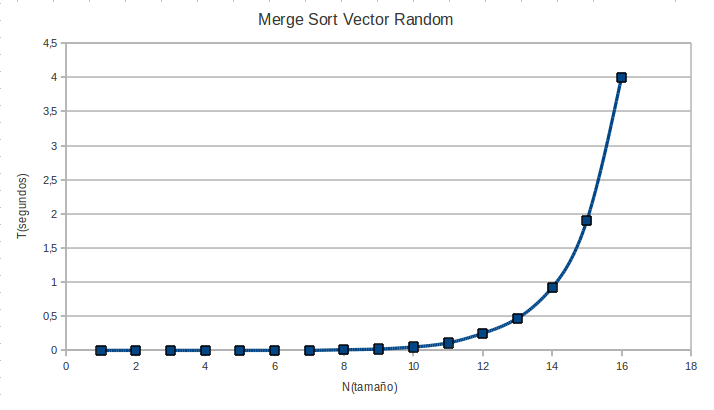
\includegraphics[width=10cm]{Imagenes/MergeSortVectorRandom.PNG}
\end{center}
\end{figure} 

\begin{figure}[!htp]
\begin{center}
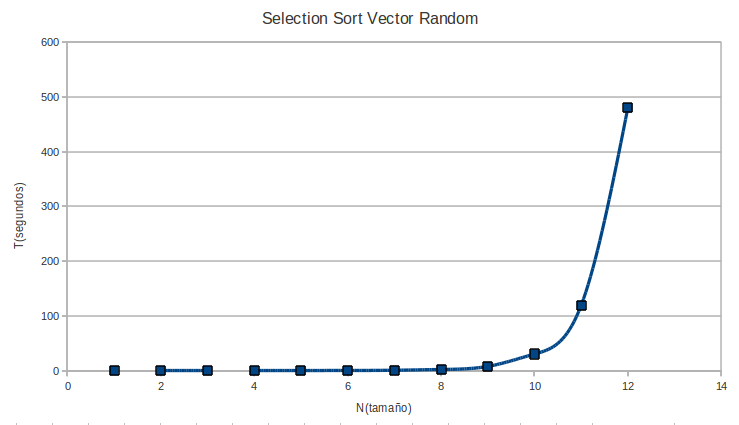
\includegraphics[width=10cm]{Imagenes/SelectionSortVectorRandom.PNG}
\end{center}
\end{figure} 

\newpage

\begin{figure}[!htp]
\begin{center}
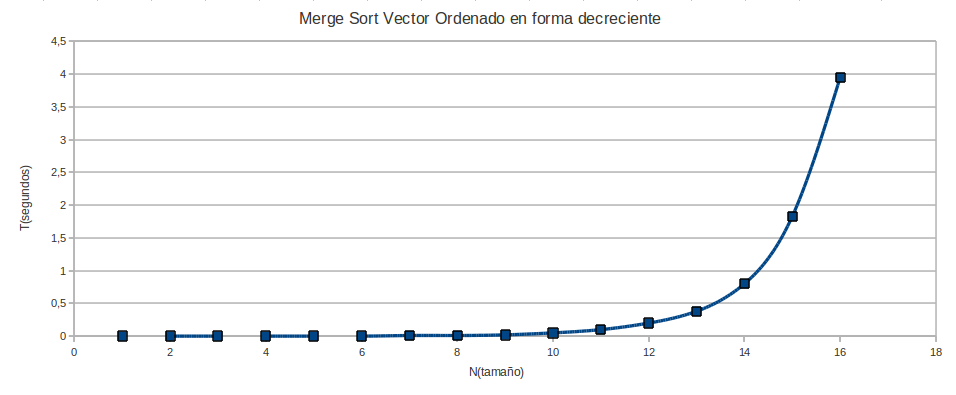
\includegraphics[width=12cm]{Imagenes/MergeSortOrdenadodecreciente.PNG}
\end{center}
\end{figure} 

\begin{figure}[!htp]
\begin{center}
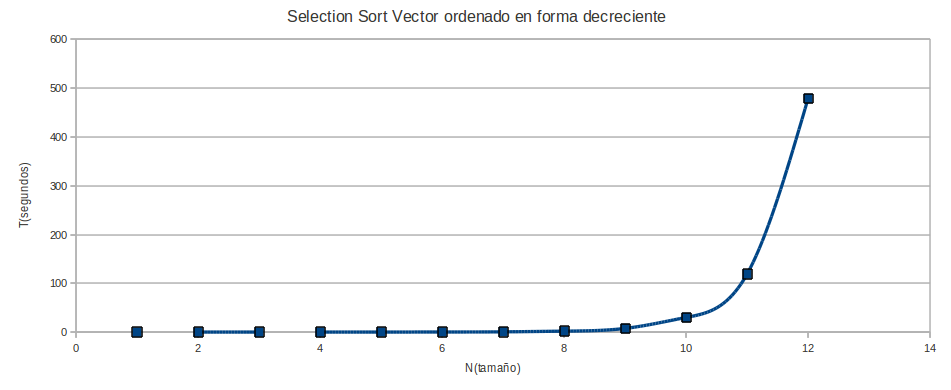
\includegraphics[width=12cm]{Imagenes/SelectionSortOrdenadodecreciente.PNG}
\end{center}
\end{figure} 

\begin{figure}[!htp]
\begin{center}
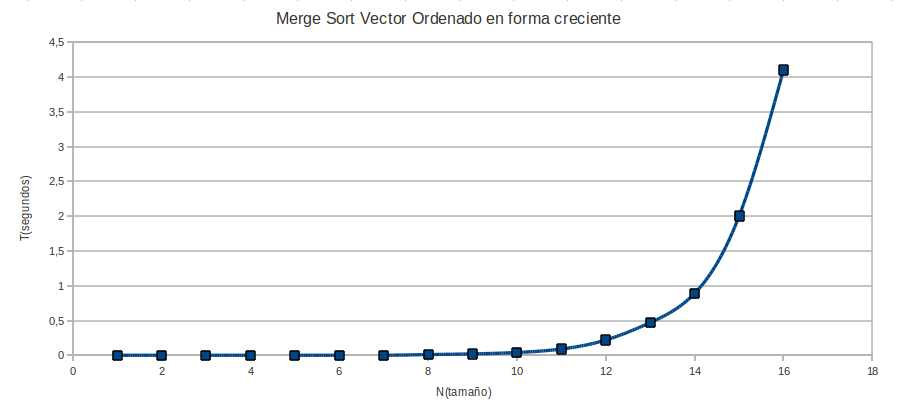
\includegraphics[width=12cm]{Imagenes/MergeSortOrdenadocreciente.PNG}
\end{center}
\end{figure} 

\begin{figure}[!htp]
\begin{center}
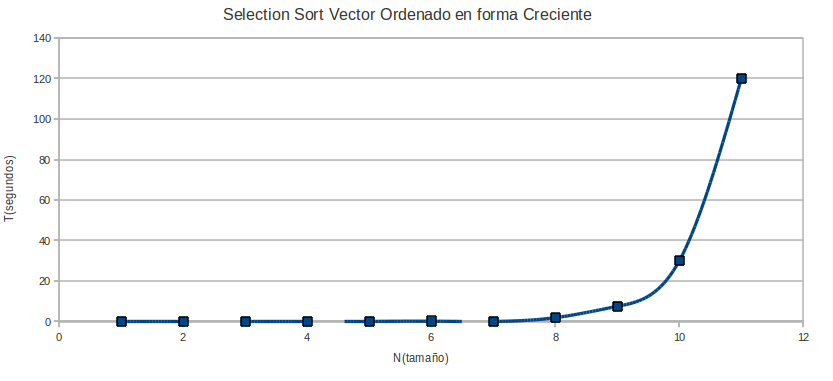
\includegraphics[width=12cm]{Imagenes/SelectionSortordenadocreciente.PNG}
\end{center}
\end{figure} 

\newpage


\subsection{Analisis de las mediciones de tiempo}
Es fácil ver que se verifica lo que se esperaba : que los 2 métodos de ordenamiento mantienen su orden de complejidad independientemente
de como se encuentra el vector. Es fácil observar también que el Merge Sort es muchísimo mas rápido que el Selection Sort.
\\Cuando N tiende a números grandes, fue imposible medir el tiempo para terminar de ordenar un vector con Selection Sort, se detuvo la medición al pasar mas de 10 minutos. Para N chicos, los 2 métodos son similares.
\\Usando estos valores, se consiguieron los Speed Up de Merge Sort vs Selection Sort.
\\$SpeedUpMs=TiempoMergeSort/TiempoSelectionSort$
Vale mencionar que para N chicos, donde los tiempos de ambos métodos son 0 o casi 0, se considera el Speed Up nulo, indicando que los 2 métodos tardaron lo mismo.
A continuacion, los graficos de los Speed Up para los distintos N, segun la forma en la que se encuentra el vector a ordenar.

\begin{figure}[!htp]
\begin{center}
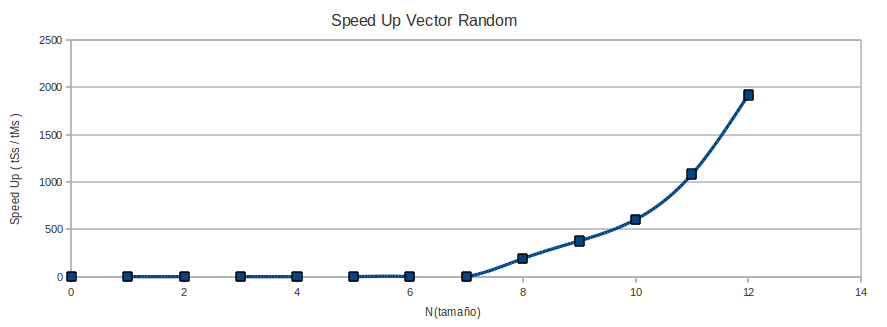
\includegraphics[width=12cm]{Imagenes/SpeedUpVectorRandom.png}
\end{center}
\end{figure} 

\begin{figure}[!htp]
\begin{center}
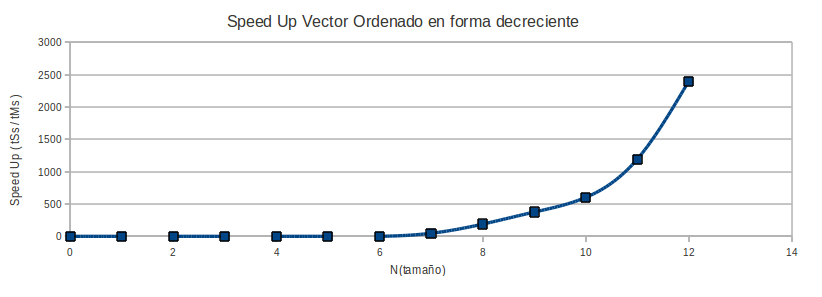
\includegraphics[width=12cm]{Imagenes/SpeedUpVectorOrdenadoEnFormaDecreciente.png}
\end{center}
\end{figure} 


\begin{figure}[!htp]
\begin{center}
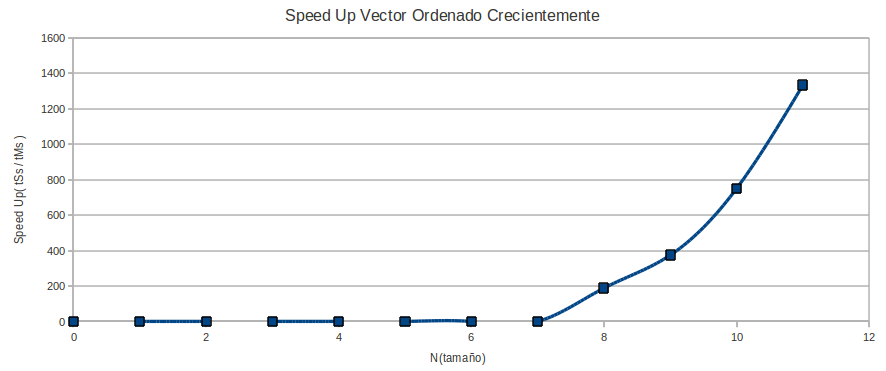
\includegraphics[width=11cm]{Imagenes/SpeedUpVectorOrdenadoEnFormaCreciente.png}
\end{center}
\end{figure} 

\newpage

Para los casos donde $N>12$ , el tiempo del Merge Sort es mas de 2 ordenes de magnitud menor que el de Selection Sort , el Speed Up crece vertiginosamente.
Se ve que los speed up varian segun los distintos casos. Esto no deberia suceder, y se debe hay otras aplicaciones corriendo mientras
se mide la performance de los algoritmos de ordenamiento,lo cual introduce algo de error en las mediciones.

\newpage

\section{Profiling con Gprof}
\subsection{Mediciones de tiempo}
Con lo dicho en los puntos anteriores, vemos que:
\begin{enumerate} 
 \item {Merge Sort es mucho mas rapido que Selection Sort}
 \item {Para casos muy grandes, no se pueden estimar los tiempos del Selection Sort, ya que da valores cercanos a las horas}
 \item {Para casos muy chicos, los algoritmos se comportan de forma similar}
\end{enumerate}
Debido a esto, elegimos un caso medio, donde $N = 10$ . Vamos a usar un vector random y la herramienta Gprof.
Vale aclarar que para poder usar esta herramienta, tuvimos que haber compilado nuestro programa con el flag -pg .
Mas adelante se vera en mas profunidad los comandos usados para compilar el codigo source en C .
\\ El gprof nos entrega un texto. Aqui se reproducen solo las partes importantes.

\verbatiminput{ArchivoDeLog.txt}


\begin{thebibliography}{9}

	\bibitem{lamport94}
	  Leslie Lamport,
	  \emph{\LaTeX: A Document Preparation System}.
	  Addison Wesley, Massachusetts,
	  2nd Edition,
	  1994.

\end{thebibliography}

\end{document}          
